\documentclass[tikz, border=10pt]{standalone}
\usepackage{amsmath}
\usepackage{amssymb}

% TikZ Libraries
\usetikzlibrary{
    arrows.meta,
    positioning,
    calc,
    shapes.geometric,
    shapes.misc,
    backgrounds,
    fit,
    shadows,
    decorations.pathreplacing
}

% Define Colors
\definecolor{p1header}{RGB}{43, 101, 152}   % Steel Blue
\definecolor{p1bg}{RGB}{229, 242, 255}      % Light Blue
\definecolor{p2header}{RGB}{198, 112, 26}   % Burnt Orange
\definecolor{p2bg}{RGB}{255, 239, 224}      % Light Orange
\definecolor{p3header}{RGB}{106, 58, 126}   % Deep Purple
\definecolor{p3bg}{RGB}{244, 232, 252}      % Light Purple
\definecolor{jsonbg}{RGB}{219, 240, 226}    % Light Green
\definecolor{jsontxt}{RGB}{30, 80, 40}      % Dark Green text

\begin{document}

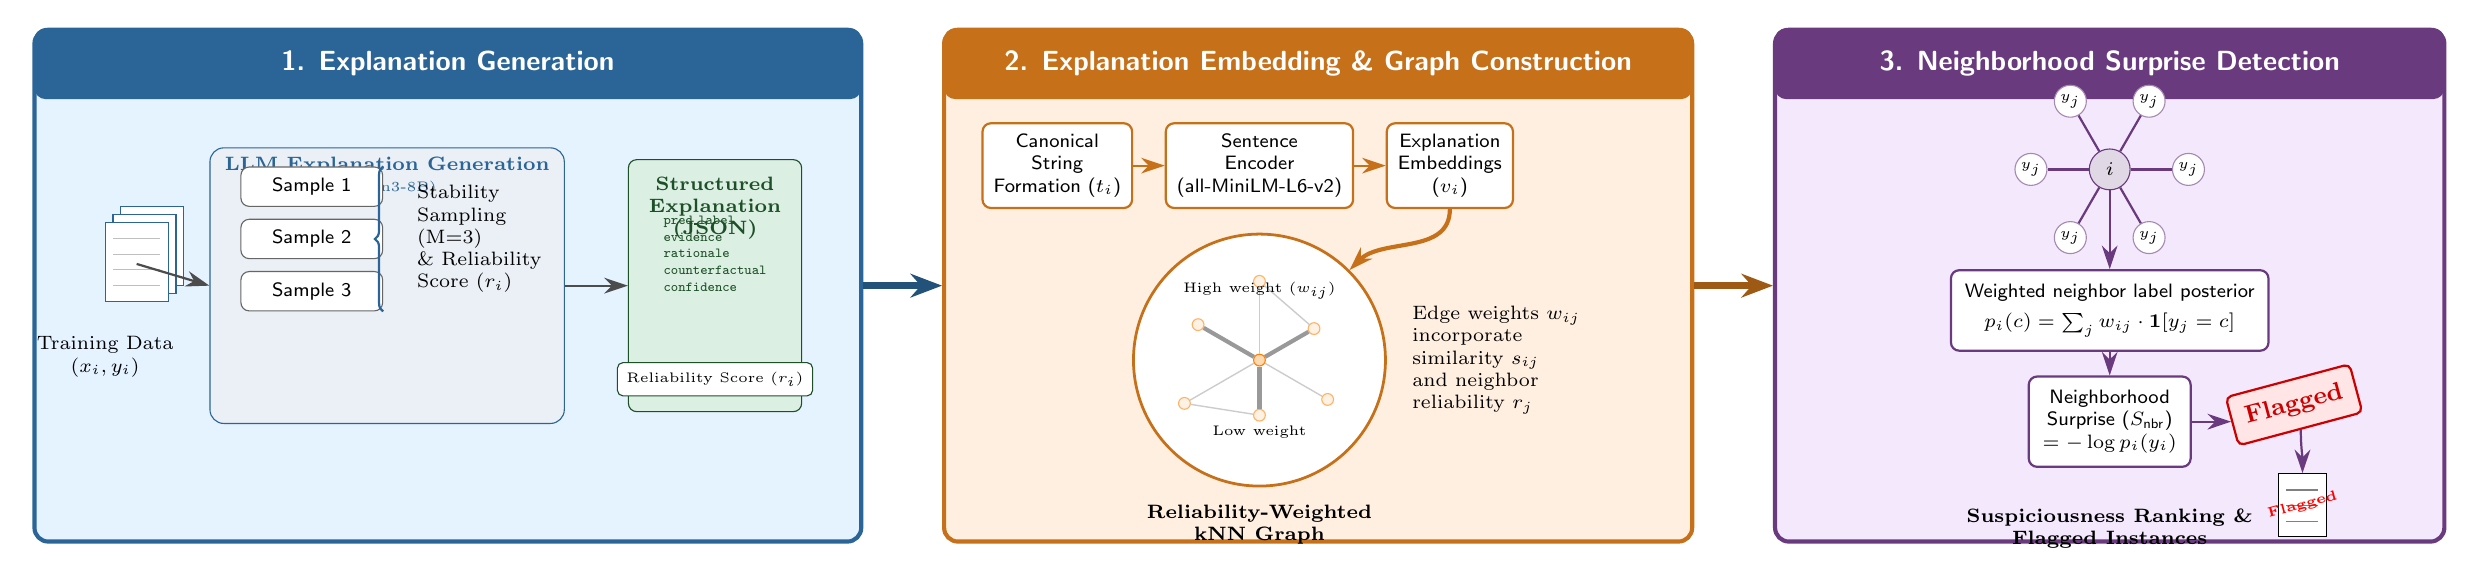
\begin{tikzpicture}[
    node distance=0.5cm,
    font=\sffamily,
    % Styles for main components
    panel/.style={
        draw=#1,
        fill=#1!15, % lighter version of border if not overridden
        line width=1.5pt,
        rounded corners=5pt,
        inner sep=0pt
    },
    header/.style={
        fill=#1,
        text=white,
        font=\bfseries\sffamily,
        align=center,
        minimum height=0.9cm,
        anchor=north,
        rounded corners=4pt
    },
    % Styles for internal boxes
    processbox/.style={
        draw=black!60,
        fill=white,
        rounded corners=3pt,
        align=center,
        font=\scriptsize\sffamily,
        inner sep=4pt
    },
    orangebox/.style={
        draw=p2header,
        fill=white,
        line width=0.8pt,
        rounded corners=3pt,
        align=center,
        font=\scriptsize\sffamily,
        inner sep=4pt
    },
    purplebox/.style={
        draw=p3header,
        fill=white,
        line width=0.8pt,
        rounded corners=3pt,
        align=center,
        font=\scriptsize\sffamily,
        inner sep=5pt
    },
    % Arrow Styles
    arrow/.style={
        ->,
        >={Stealth[length=3mm, width=2mm]},
        thick,
        draw=black!70
    },
    panelarrow/.style={
        ->,
        >={Stealth[length=4mm, width=3mm]},
        line width=2.5pt,
        draw=#1
    }
]

% ==========================================================================================
% PANEL 1: Explanation Generation
% ==========================================================================================

% Background & Header
\node[panel=p1header, fill=p1bg, minimum width=10.5cm, minimum height=6.5cm] (P1) at (0,0) {};
\node[header=p1header, minimum width=10.5cm] (H1) at (P1.north) {1. Explanation Generation};

% 1. Training Data Icon (Left)
\node[anchor=west] (data_center) at ($(P1.west)+(0.8, -0.2)$) {};

% Draw stylized document stack
\foreach \x/\y in {0.2/0.2, 0.1/0.1, 0/0} {
    \draw[fill=white, draw=p1header] ($(data_center)+(\x,\y)$) rectangle ++(0.8, 1.0);
    \foreach \l in {0.2, 0.4, 0.6, 0.8} {
        \draw[gray!50] ($(data_center)+(\x+0.1,\y+1.0-\l)$) -- ++(0.6,0);
    }
}
\node[below=0.2cm of data_center, align=center, font=\scriptsize] (data_label) {Training Data\\$(x_i, y_i)$};

% 2. LLM Box (Center)
\node[draw=p1header, fill=p1header!10, rounded corners=5pt, 
      minimum width=4.5cm, minimum height=3.5cm, 
      right=1.2cm of data_center, yshift=0.2cm] (llm_container) {};

\node[anchor=north, font=\bfseries\scriptsize, text=p1header] at (llm_container.north) {LLM Explanation Generation};
\node[anchor=north, font=\tiny, text=p1header, yshift=-0.3cm] at (llm_container.north) {(Qwen3-8B)};

% Samples inside LLM
\node[processbox, minimum width=1.8cm, yshift=-0.5cm] (s1) at (llm_container.north west) [xshift=1.3cm] {Sample 1};
\node[processbox, minimum width=1.8cm, below=0.15cm of s1] (s2) {Sample 2};
\node[processbox, minimum width=1.8cm, below=0.15cm of s2] (s3) {Sample 3};

% Brace and Text
\draw[decorate, decoration={brace, amplitude=3pt, mirror}, thick, p1header] 
    (s1.north east) -- (s3.south east) coordinate[midway, xshift=3pt] (brace_mid);

\node[right=0.2cm of brace_mid, align=left, font=\scriptsize, text width=1.8cm] {Stability\\Sampling (M=3)\\\& Reliability\\Score ($r_i$)};

% 3. Structured Explanation (Right)
\node[draw=jsontxt, fill=jsonbg, rounded corners=3pt, 
      right=0.8cm of llm_container, 
      minimum width=2.2cm, minimum height=3.2cm, align=left, font=\scriptsize] (json_box) {};

\node[anchor=north, font=\bfseries\scriptsize, text=jsontxt, align=center, yshift=-0.1cm] at (json_box.north) {Structured\\Explanation\\(JSON)};

% JSON Content
\node[below=0.6cm of json_box.north, anchor=north, align=left, font=\ttfamily\tiny, text=jsontxt] {
    pred\_label\\
    evidence\\
    rationale\\
    counterfactual\\
    confidence
};

% Reliability Score sub-box
\node[draw=jsontxt, fill=white, rounded corners=2pt, font=\tiny, anchor=south, yshift=0.2cm] at (json_box.south) {Reliability Score ($r_i$)};

% Arrows Panel 1
\draw[arrow] (data_label.north) ++(0.4, 0.8) -- (llm_container.west);
\draw[arrow] (llm_container.east) -- (json_box.west);


% ==========================================================================================
% PANEL 2: Embedding & Graph
% ==========================================================================================

% Background & Header
\node[panel=p2header, fill=p2bg, minimum width=9.5cm, minimum height=6.5cm, right=1.0cm of P1] (P2) {};
\node[header=p2header, minimum width=9.5cm] (H2) at (P2.north) {2. Explanation Embedding \& Graph Construction};

% 1. Pipeline Row (Top)
\node[orangebox, anchor=north west] (canon) at ($(P2.north west)+(0.5, -1.2)$) {Canonical\\String\\Formation ($t_i$)};
\node[orangebox, right=0.4cm of canon] (enc) {Sentence\\Encoder\\(all-MiniLM-L6-v2)};
\node[orangebox, right=0.4cm of enc] (emb) {Explanation\\Embeddings\\($v_i$)};

\draw[arrow, color=p2header] (canon) -- (enc);
\draw[arrow, color=p2header] (enc) -- (emb);

% 2. kNN Graph (Center Bottom)
\node[circle, draw=p2header, fill=white, line width=1pt, minimum size=3.2cm, below=0.3cm of enc] (graph_circle) {};

% Graph Nodes
\begin{scope}[shift={(graph_circle.center)}]
    % Nodes
    \node[circle, fill=orange!30, draw=orange, inner sep=1.5pt] (c) at (0,0) {}; % Center
    \foreach \angle/\dist/\n in {30/0.8/1, 90/1.0/2, 150/0.9/3, 210/1.1/4, 270/0.7/5, 330/1.0/6} {
        \node[circle, fill=orange!10, draw=orange!60, inner sep=1.5pt] (n\n) at (\angle:\dist) {};
    }
    
    % Edges (thick = high weight, thin = low weight)
    \draw[line width=1.5pt, gray!80] (c) -- (n1);
    \draw[line width=1.5pt, gray!80] (c) -- (n3);
    \draw[line width=0.5pt, gray!40] (c) -- (n2);
    \draw[line width=0.5pt, gray!40] (c) -- (n4);
    \draw[line width=1.5pt, gray!80] (c) -- (n5);
    \draw[line width=0.5pt, gray!40] (c) -- (n6);
    
    % Inter-neighbor edges
    \draw[line width=0.5pt, gray!40] (n1) -- (n2);
    \draw[line width=0.5pt, gray!40] (n4) -- (n5);
\end{scope}

% Annotations
\node[below=0.1cm of graph_circle, font=\bfseries\scriptsize, align=center] {Reliability-Weighted\\kNN Graph};

% Legendish text inside circle (simulated position)
\node[font=\tiny, anchor=north] at ($(graph_circle.north)+(0,-0.5)$) {High weight ($w_{ij}$)};
\node[font=\tiny, anchor=south] at ($(graph_circle.south)+(0,0.5)$) {Low weight};

% Side Text
\node[right=0.2cm of graph_circle, font=\scriptsize, text width=2.5cm, align=left] {Edge weights $w_{ij}$\\incorporate\\similarity $s_{ij}$\\and neighbor\\reliability $r_j$};

% Arrow pipeline to graph
\draw[arrow, color=p2header, line width=1.5pt] (emb.south) to[out=270, in=45] (graph_circle.45);

% Connect Panel 1 to Panel 2 (Logical flow)
\draw[panelarrow=p1header!80!black] (P1.east) -- (P2.west);


% ==========================================================================================
% PANEL 3: Surprise Detection
% ==========================================================================================

% Background & Header
\node[panel=p3header, fill=p3bg, minimum width=8.5cm, minimum height=6.5cm, right=1.0cm of P2] (P3) {};
\node[header=p3header, minimum width=8.5cm] (H3) at (P3.north) {3. Neighborhood Surprise Detection};

% 1. Star Graph (Top)
\node[circle, fill=p3header!20, draw=p3header, font=\scriptsize] (center_node) at ($(P3.north)+(0,-1.8)$) {$i$};
\foreach \angle in {0, 60, 120, 180, 240, 300} {
    \node[circle, fill=white, draw=p3header!60, inner sep=1pt, font=\tiny] (leaf\angle) at ($(center_node)+(\angle:1.0)$) {$y_j$};
    \draw[thick, p3header] (center_node) -- (leaf\angle);
}

% 2. Formula Boxes
% Posterior
\node[purplebox, below=0.5cm of center_node, yshift=-0.5cm] (posterior) {
    Weighted neighbor label posterior\\[3pt]
    $p_i(c) = \sum_j w_{ij} \cdot \mathbf{1}[y_j = c]$
};

% Surprise
\node[purplebox, below=0.3cm of posterior] (surprise) {
    Neighborhood\\Surprise ($S_{\text{nbr}}$)\\$= -\log p_i(y_i)$
};

% 3. Flagged Badge
\node[draw=red!80!black, fill=red!10, thick, rounded corners=2pt, rotate=15, 
      right=0.5cm of surprise, font=\bfseries\small, text=red!80!black, inner sep=5pt] (flagged) {Flagged};

\draw[arrow, color=p3header] (surprise.east) -- (flagged.west);

% 4. Output Label
\node[below=0.4cm of surprise, font=\bfseries\scriptsize, align=center] (output) {Suspiciousness Ranking \&\\Flagged Instances};

% List Icon next to output
\node[draw=black, fill=white, minimum width=0.6cm, minimum height=0.8cm, right=0.2cm of output, yshift=0.3cm] (listicon) {};
\foreach \y in {0.2, 0.4, 0.6} {
    \draw[gray] ($(listicon.south west)+(0.1,\y)$) -- ++(0.4,0);
}
% Red cross/stamp on icon
\node[text=red, font=\bfseries\tiny, rotate=15] at (listicon.center) {Flagged};

% Connect Panel 2 to Panel 3
\draw[panelarrow=p2header!80!black] (P2.east) -- (P3.west);

% Connect Graph Components inside Panel 3
\draw[arrow, color=p3header] (center_node.south) -- (posterior.north);
\draw[arrow, color=p3header] (posterior.south) -- (surprise.north);
\draw[arrow, color=p3header] (flagged.south) to[out=270, in=90] (listicon.north);

\end{tikzpicture}

\end{document}

